\documentclass[../../../../main.tex]{subfiles}
\begin{document}

\begin{flushright}
\footnotesize\textit{【自動文字起こし・要確認】}
\end{flushright}

\noindent
\textbf{[解]} (1) 正六角形であるから右図。

\begin{center}
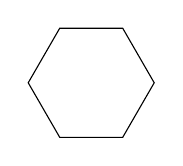
\begin{tikzpicture}[scale=0.8]
  \draw (0:1) -- (60:1) -- (120:1) -- (180:1) -- (240:1) -- (300:1) -- cycle;
\end{tikzpicture}
\end{center}

\bigskip

\noindent
(2) 正八面体の6頂点 $A \sim F$ とし、右図のように面 ABC, 面 DEF の重心を $G_1, G_2$ とする。直線 $G_1 G_2$ を $l$ とおく。$l$ は面 ABC, 面 DEF と垂直である。$\vec{G_1 G_2} = \vec{a}$ とおき、$\vec{G_1 P} = t \vec{a} \; (0 \le t \le 1)$ なる点 $P$ を含み $l$ に垂直な平面で立体を切断する。この時の断面は右図。この時、右図のように頂点をおくと、相似から
\[
\begin{cases}
\overline{LK} = \overline{MH} = \overline{IJ} = 1-t \\
\overline{HI} = \overline{KJ} = \overline{LM} = t
\end{cases}
\]
（$H$ は $BD$ 上、$I$ は $BE$ 上、$J$ は $CE$ 上、$K$ は $CF$ 上）\\
となり、これを回転させた面積 $S(t)$ は
\[
S(t) = \pi \cdot \overline{PJ}^2 \quad \cdots \text{①}
\]
である。右上図から、
\[
\overline{PJ}^2 = \left(\frac{1}{2}t\right)^2 + \left\{ \frac{\sqrt{3}}{2}(2-t) \right\}^2 = \frac{1}{12}(4t^2 - 4t + 4) = \frac{1}{3}(t^2 - t + 1)
\]
だから、①に代入して
\[
S(t) = \frac{\pi}{3}(t^2 - t + 1)
\]
である。$\overline{G_1 G_2} = \frac{\sqrt{6}}{3}$ だから求める体積 $V$ は
\begin{align*}
V &= \int_0^1 \frac{\pi}{3}(t^2 - t + 1) \cdot \frac{\sqrt{6}}{3} \, dt \\
&= \frac{\sqrt{6}\pi}{9} \left[ \frac{1}{3}t^3 - \frac{1}{2}t^2 + t \right]_0^1 \\
&= \frac{5\sqrt{6}}{54}\pi \hfill \text{\#}
\end{align*}

\bigskip

\begin{center}
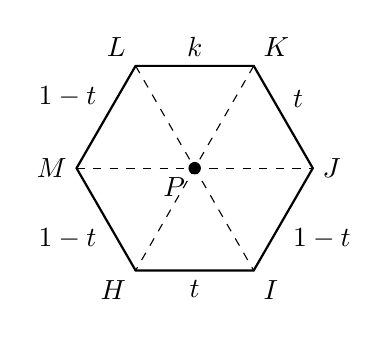
\begin{tikzpicture}[scale=1.5, >=stealth]
  \coordinate (P) at (0,0);
  \coordinate (L) at (-0.5, 0.866);
  \coordinate (K) at (0.5, 0.866);
  \coordinate (J) at (1, 0);
  \coordinate (I) at (0.5, -0.866);
  \coordinate (H) at (-0.5, -0.866);
  \coordinate (M) at (-1, 0);

  \draw[thick] (L) -- (K) -- (J) -- (I) -- (H) -- (M) -- cycle;
  \draw[dashed] (L) -- (I);
  \draw[dashed] (K) -- (H);
  \draw[dashed] (M) -- (J);

  \fill (P) circle (1.5pt) node[below left] {$P$};
  \node[above left] at (L) {$L$};
  \node[above right] at (K) {$K$};
  \node[right] at (J) {$J$};
  \node[below right] at (I) {$I$};
  \node[below left] at (H) {$H$};
  \node[left] at (M) {$M$};

  \node[above] at (0, 0.866) {$k$};
  \node[above right] at (0.75, 0.433) {$t$};
  \node[below right] at (0.75, -0.433) {$1-t$};
  \node[below] at (0, -0.866) {$t$};
  \node[below left] at (-0.75, -0.433) {$1-t$};
  \node[above left] at (-0.75, 0.433) {$1-t$};
\end{tikzpicture}
\end{center}

\bigskip

\noindent
\textbf{[解2]} (2) $G_1 G_2$ の中点を $O$ とし、$\triangle OAG_1$ に三平方の定理を用いて
\[
\overline{OG_1}^2 = \left(\frac{\sqrt{2}}{2}\right)^2 - \left(\frac{\sqrt{3}}{3}\right)^2 = \frac{1}{6}
\]
だから、
\[
\overline{G_1 G_2} = 2\sqrt{\frac{1}{6}} = \frac{\sqrt{6}}{3} \quad \cdots \text{①}
\]
である。[解1]と同様にして、切断面は右図。
余弦定理から、
\begin{align*}
\overline{PH}^2 &= \left(\frac{\sqrt{3}}{3}\right)^2 + \left(\frac{\sqrt{3}}{3}t\right)^2 - 2 \cdot \frac{\sqrt{3}}{3} \cdot \frac{\sqrt{3}}{3}t \cos 60^\circ \\
&= \frac{1}{3}(t^2 - t + 1)
\end{align*}
(以下略)

\end{document}
